\documentclass[11pt]{article}

\usepackage[T1]{fontenc}
\usepackage{lmodern}
\usepackage[margin=1.15in]{geometry}
\usepackage{amsmath,amssymb,amsthm}
\usepackage{setspace}
\usepackage[hidelinks]{hyperref}
\usepackage{tikz}
\usetikzlibrary{arrows.meta,positioning,shapes.geometric}

\newtheorem{proposition}{Proposition}
\theoremstyle{remark}
\newtheorem*{remark}{Remark}

\setstretch{1.08}
\setlength{\parskip}{0.55em}
\setlength{\parindent}{0pt}

\title{Beyond the Token Budget:\\[0.3em]
\large Formal Reasoning, Representation, and the Economics of Computational Scale}
\author{Flyxion\\ \small Independent Researcher}
\date{October 2026}

\begin{document}
\maketitle

\begin{abstract}
\noindent
Capability does not close the resource problem in computational research, because each working method suggests a larger application and the supply of worthwhile applications grows faster than the means of executing them. This essay treats the token budget as a design constraint rather than a temporary inconvenience and asks what kind of research system remains useful under it. Four claims are developed. First, formal writing is a form of computation performed in advance, valuable to the extent that it proves, prunes, or rules out, and not merely because it names. Second, a compressed representation should be judged by the distinctions it keeps available to a particular consumer, a point supported by recent evidence that numerical reconstruction error and downstream usefulness can diverge sharply. Third, correction should be delivered in a form the learner can absorb, a point supported by a cross-paradigm distillation study in which a stronger teacher degraded the student when its predictions were imposed directly, and improved it when the student's own predictions mediated the transfer. Fourth, retained experience has to be usable as well as stored, a point supported by a study of agents that pair an external memory of strategy cards with a continually trained adapter, and which suggests a progression from interpreted guidance to checked, executable procedures. A supporting technical observation is that the treatment of absent information differs systematically between programming languages, data libraries, and symbolic systems, and that these conventions supply a precise vocabulary for the way a model fills a state for which no attested form exists. The essay closes with an accounting of reuse and a set of measurable quantities for resource-constrained research systems, together with worked symbolic examples and an explicit statement of what the cited evidence does and does not establish.
\end{abstract}

\section{Demand That Grows With Capability}

The difficulty with computational research is usually described as a shortage of capability. A model cannot reason well enough, a machine cannot run a sufficiently large network, or a software environment lacks the tools a task requires. Yet a second difficulty appears as soon as these capabilities become useful: the supply of worthwhile applications grows faster than the resources available to execute them. A working method immediately suggests a larger experiment. An effective document analysis invites application to an entire archive. A successful programming assistant suggests a system that examines every repository, tests every implementation, and compares every plausible alternative. Under these conditions improved capability does not settle the resource problem. It enlarges the territory over which that problem operates.

Language-model infrastructure makes the difficulty concrete. A sophisticated harness can coordinate tools, manage context, assign subtasks, and revise an answer repeatedly, but each additional operation consumes tokens. When generation is constrained, whether by subscription limits, API expenditure, local throughput, memory, or electricity, orchestration has to justify its own cost. A harness may make an individual task more reliable while making the larger research programme less affordable. The appropriate unit of evaluation is therefore the useful work completed across the programme, including the opportunities forgone when its resources are exhausted. The pace at which a metered service can be consumed is itself instructive: agentic coding routinely accounts for very large token volumes, and a method that proves effective on one repository invites immediate application to all of them.

Seeking a local model addresses part of this. Local inference gives control over execution and reduces dependence on a metered service, but it does not make computation unlimited. Accelerator memory, generation speed, hardware expenditure, and maintenance remain constraints. A more durable aim is to perform the necessary work with fewer model calls, smaller representations, ordinary processors where feasible, and procedures whose cost stays manageable as the archive grows. Independence from specialized accelerators is an architectural aspiration whose feasibility has to be established task by task, and the sections below are largely concerned with how such establishment might proceed.

\section{Accounting for Scale}

It is easy to underestimate demand by imagining a fixed collection of requests. A researcher with an extensive archive does not face a single immutable task count, because the number of tasks depends on how the material is divided and which relationships are investigated. Five hundred documents can become ten thousand passages, a million claims, or a far larger set of candidate comparisons. Parsing is already an experimental decision, since it determines the objects over which later computation operates.

A simple accounting makes the structure visible. If $N$ units each require on average $k$ model calls, with average input and output lengths $I$ and $O$, the uncached token volume is approximately
\begin{equation}
T \approx N\,k\,(I+O).
\end{equation}
Every factor can expand. Documents acquire annotations, annotations become inputs to comparisons, and failed comparisons generate requests for clarification. A harness can increase $k$, and repeatedly supplying background material increases $I$. If the task calls for unrestricted pairwise comparison, the number of candidate relationships is
\begin{equation}
\binom{N}{2} = \frac{N(N-1)}{2},
\end{equation}
which grows quadratically while the archive grows linearly. Lowering the price of a token helps, but it leaves this structure intact. A research system also needs ways to avoid processing irrelevant relationships, to avoid repeating established work, and to avoid reconstructing information it already holds.

Future income does not remove the concern. Additional revenue can purchase more computation, but a researcher who readily enlarges a problem can exhaust a larger budget almost as readily as a smaller one. The enduring question is how expenditure relates to durable knowledge. Consider a programme of $m$ investigations. Investigation $j$ would cost $a_j$ tokens if begun from nothing. Suppose retained artefacts from earlier work already avoid a fraction $r_j \in [0,1]$ of that baseline expenditure, and suppose that making the outputs of investigation $j$ reusable (linking them to sources, checking them, recording their assumptions) costs an additional $s_j$, which also includes the retrieval, applicability checking, and maintenance that reuse requires, counted once. The total cost is then
\begin{equation}
C \;=\; \sum_{j=1}^{m}\bigl[(1-r_j)\,a_j + s_j\bigr],
\qquad
C_0 \;=\; \sum_{j=1}^{m} a_j ,
\end{equation}
where $C_0$ is the cost with no retention. The fraction $r_j$ measures expenditure avoided and not questions answered, and the two agree only when every question costs the same. If an investigation contains ten questions and would cost 10{,}000 tokens, with nine questions costing 100 tokens each and the tenth costing 9{,}100, then reusing the answers to the nine inexpensive questions answers 90 percent of the questions but avoids only 900 tokens, so $r_j = 0.09$ and 9{,}100 tokens of work remain before overhead. Retention pays exactly when $\sum_j s_j < \sum_j r_j a_j$. This is an accounting identity and not a result, but it locates the questions that matter. The reuse fractions $r_j$ depend on whether stored artefacts preserve the distinctions later questions need, which is a question about representation. The overhead $s_j$ depends largely on how cheaply outputs can be verified and corrected, which is a question about the interface between a strong source of correction and the system that must absorb it. Both are taken up below, after sections on what can be done before any model is called, and Section~\ref{sec:measure} describes how $r_j$ and $s_j$ could be estimated on a real archive.

\section{Formal Writing as Computation Performed in Advance}

An essay can carry out substantial conceptual work before a programme is written. Definitions specify admissible objects. Assumptions identify the conditions under which a procedure is supposed to operate. A proof can establish a property for an entire class of cases, and a counterexample can show that a proposed implementation cannot achieve its stated objective without added restrictions. These activities can prevent expensive experiments whose outcomes were already determined by their premises. Mathematical notation also serves as a compact specification of computation: a recurrence describes an iterative process, an operator describes a transformation, and an invariant states what execution must preserve. Some formal systems admit direct execution or mechanized checking, and others remain descriptions from which implementations have to be developed. In either case symbolic work can expose dependencies and contradictions that would otherwise surface only after substantial engineering.

The savings require a qualification. Writing an expression for a difficult operation does not perform it. Defining an optimum does not supply an efficient search, and naming a repair operator does not establish that repair is computable or convergent. Formal writing earns its computational value when it proves something, shrinks a search space, identifies an impossibility, or makes an implementation obligation precise. Its strongest contribution is often to determine which calculations deserve to be run.

A small example shows the kind of result that earns this value. Let an archive contain records $x \in X$, and let a compression scheme assign each record a code of $B$ bits. Let $q : X \to Y$ be the function that answers some family of future questions.

\begin{proposition}
If $q$ takes more than $2^{B}$ distinct values on $X$, then no procedure that sees only the $B$-bit codes can compute $q$ correctly on all of $X$, whatever model or amount of computation is applied downstream.
\end{proposition}

\begin{proof}
There are at most $2^{B}$ distinct codes. If $q$ takes more than $2^{B}$ values, two records with different $q$-values must share a code, and any procedure that sees only the code returns the same answer for both, so it is wrong on at least one of them.
\end{proof}

The proposition is an elementary bookkeeping observation, and its later invocations are illustrative and not load-bearing, which is part of its use. It states in advance that no quantity of downstream inference recovers a distinction the representation has discarded, so an archive must be compressed for the questions it is expected to serve, and the cost of a wrong guess about those questions is paid at query time. It also fixes the meaning of a nominal bit budget as a ceiling on distinguishability, not as a measure of what a consumer can in fact use. The statement is the contrapositive of the requirement that distinct answers have distinct codes, and its later invocations in the sections on representation, absence, and retrieval are deliberate repetitions of the same ceiling argument. Later sections turn to evidence on how far a real system sits below that ceiling.

For research under resource constraints, this suggests a productive sequence. Symbolic analysis establishes the structure of the question. Small experiments test the assumptions most likely to fail. Larger execution follows when the earlier stages supply a reason to expect informative results. Essays therefore function as intermediate research artefacts that preserve reasoning while postponing expenditure.

\section{Symbolic Computation Before Pipeline Execution}

Computer algebra supplies a practical precedent for treating formal reasoning as part of computation itself. A conventional numerical programme commonly describes operations to perform on supplied values. A symbolic programme can instead represent the expression governing those operations and transform it before particular values are supplied. SymPy \cite{meurer2017} makes this distinction tangible: an expression becomes an inspectable mathematical object, allowing the system to derive a simpler calculation, establish an identity, or produce a reusable formula.

A related computational precedent is partial evaluation \cite{futamura1999}. When some inputs to a programme are already known, the operations determined by those inputs can be performed in advance, leaving a specialized programme for the inputs that remain unknown. Writing $P(s,d)$ for a programme with fixed information $s$ and later data $d$, specialization seeks a residual programme $P_s$ satisfying
\begin{equation}
P_s(d) = P(s,d)
\end{equation}
on the specified domain. The work performed during specialization is justified by subsequent executions that no longer repeat it. This is a precise precedent for the essay's economic argument, although an informal mathematical derivation is not automatically a semantics-preserving programme transformation. Its assumptions, exceptional cases, and correspondence with the residual implementation remain obligations to establish.

Consider a research process in which the cost of processing successive documents grows because each document receives an increasing amount of context. Suppose the first document costs $a$ tokens and each subsequent document costs an additional $b$ tokens. An object-oriented implementation might construct a processing job for each document and accumulate its estimated cost. A functional implementation might map a cost function over the document indices and reduce the resulting sequence:
\begin{verbatim}
def total_cost(n, a, b):
    return sum(a + b*i for i in range(n))
\end{verbatim}
Both approaches evaluate the individual terms, and the limitation belongs to term-by-term evaluation and not to either programming paradigm: an object-oriented or a functional programme can implement the derived closed form equally well once it is available, and functional composition is in fact a natural way to express and combine the symbolic transformations themselves, as the composition example below shows. A symbolic formulation exposes the structure of the whole calculation:
\begin{verbatim}
import sympy as sp

i = sp.symbols("i", integer=True)
n = sp.symbols("n", integer=True, positive=True)
a, b = sp.symbols("a b", nonnegative=True)

total = sp.summation(a + b*i, (i, 0, n - 1))
total = sp.factor(total)
\end{verbatim}
The result is the closed expression
\begin{equation}
T(n) = an + \frac{bn(n-1)}{2}.
\end{equation}
The numerical pipeline requires $n$ term evaluations for each scenario, whereas the derived expression requires a fixed number of arithmetic operations, apart from the cost of operating on larger numbers. More significantly, the formula reveals that a positive context increment introduces quadratic growth. An implementation that merely processes jobs can measure this growth, but the symbolic expression makes its cause explicit before any jobs are run. The formula applies to the stipulated cost model; it does not establish that actual token consumption follows that model.

A similar advantage appears when repeated updates have a common structure. Suppose a system repeatedly updates a quantity according to
\begin{equation}
x_{k+1} = \mu x_k + c.
\end{equation}
A direct implementation performs the recurrence step by step:
\begin{verbatim}
def advance(x, mu, c, steps):
    for _ in range(steps):
        x = mu*x + c
    return x
\end{verbatim}
A symbolic treatment separates the repeated multiplication from the accumulated additions:
\begin{verbatim}
j = sp.symbols("j", integer=True)
mu, c, x0 = sp.symbols("mu c x0")

xn = mu**n*x0 + c*sp.summation(mu**j, (j, 0, n - 1))
\end{verbatim}
For $\mu \neq 1$, the corresponding expression is
\begin{equation}
x_n = \mu^n x_0 + c\,\frac{1-\mu^n}{1-\mu},
\end{equation}
while $\mu = 1$ gives $x_n = x_0 + nc$. This replaces explicit traversal of the recurrence when only its final value is required. It also exposes the conditions for convergence: for real $\mu$ with $|\mu| < 1$, the sequence approaches $c/(1-\mu)$. The symbolic calculation therefore produces both an executable shortcut and an explanation of the system's behaviour. If intermediate states trigger actions or introduce nonlinear feedback, those additional dynamics must be represented before the shortcut remains valid.

A derived closed form should itself be checked before it replaces the loop it summarizes, and SymPy can perform part of that check without running either implementation. A closed form for a recurrence is correct when it reproduces the initial value and satisfies the update rule for every index, and both conditions are algebraic statements about the expression:
\begin{verbatim}
closed = lambda m: mu**m*x0 + c*(1 - mu**m)/(1 - mu)

initial_gap = sp.simplify(closed(0) - x0)
update_gap = sp.simplify(closed(n + 1) - (mu*closed(n) + c))
\end{verbatim}
Both differences reduce to zero, so the expression is an exact solution of the stated recurrence for all $n$ and all $\mu \neq 1$, not merely for the sampled values that a numerical test would examine. For an explicitly defined recurrence with a uniquely determined trajectory, verifying the initial condition and the update identity establishes the proposed closed form by induction on its stated domain. The shortcut is accepted when its difference from the defining rule simplifies to zero, and it is sent back for revision when the residue is nonzero, in which case the residue frequently indicates which case was omitted. Other computations carry their own correctness obligations, which may include preserved state, side effects, termination, and numerical error, and symbolic equality does not certify an implementation executed in finite precision. As with the earlier caveat, a nonzero output from an incomplete simplifier is a prompt for closer inspection and is not by itself a refutation.

Symbolic differentiation provides another established example. A numerical workflow might estimate how a cost changes by repeatedly perturbing an input and rerunning the calculation. For an explicit mathematical model, SymPy can derive the sensitivity once:
\begin{verbatim}
N = sp.symbols("N", positive=True)
alpha, beta = sp.symbols("alpha beta", positive=True)

cost = alpha*N + beta*N*(N - 1)/2
marginal_cost = sp.diff(cost, N)
next_item_cost = sp.simplify(cost.subs(N, N + 1) - cost)
\end{verbatim}
These expressions distinguish continuous sensitivity from the exact cost of adding one discrete item:
\begin{equation}
\frac{dC}{dN} = \alpha + \beta\left(N - \frac{1}{2}\right),
\qquad
C(N+1) - C(N) = \alpha + \beta N.
\end{equation}
That distinction matters for an archive whose comparisons grow with its size. The symbolic model identifies the source of increasing marginal cost without executing every possible archive size. It also supplies a reusable result for budget planning. Where the underlying process is a black box rather than an explicit expression, empirical measurements or other differentiation methods remain necessary.

The same cost model can be inverted to answer a planning question directly. Given a token allowance $B$ for a run whose cost is $T(n) = an + bn(n-1)/2$, the largest number of documents that fits is the integer part of the positive root of $T(n) = B$, which a solver returns without any search over candidate values of $n$ when $n$ is first treated as a real variable and integrality is imposed afterwards, a step that is valid because the polynomial extension $T(n) = an + bn(n-1)/2$ has derivative $a + b(n - \tfrac{1}{2})$, so that $T$ is increasing over real $n \ge 1$ when $a, b \ge 0$ and not both zero:
\begin{verbatim}
B, n_real = sp.symbols("B n_real", positive=True)
roots = sp.solve(sp.Eq(a*n_real + b*n_real*(n_real - 1)/2, B), n_real)
\end{verbatim}
For $b > 0$ the admissible root is
\begin{equation}
n^{*} = \frac{b - 2a + \sqrt{(2a - b)^2 + 8bB}}{2b}, \qquad n_{\max} = \lfloor n^{*} \rfloor,
\end{equation}
and for $b = 0$ and $a > 0$ the cost is linear and $n_{\max} = \lfloor B/a \rfloor$, while for $a = b = 0$ the stipulated model imposes no finite limit. The quadratic expression can be checked on a small case: with $a = 3$, $b = 2$, and $B = 120$ it gives $n^{*} = 10$, matching the direct sum. The expression also shows how the capacity responds to the parameters. Capacity grows roughly as the square root of the allowance when the quadratic term dominates and roughly linearly when the linear term dominates, so doubling the allowance doubles the number of documents only in the second regime, and the contribution associated with $b$ dominates the cost at sufficiently large $n$. A schedule that resets the context between batches changes the model so that $b$ applies only within a batch, and the resulting capacity can be derived in the same way before any batching code is written.

Two further decisions of the kind that recur throughout the accounting above can be settled symbolically. The first is whether retaining an artefact pays. Suppose that producing a verified record costs $s$ tokens once, and that each later investigation that reuses it avoids a fraction $r$ of a task of cost $a$. The record recovers its production cost after $m$ investigations where
\begin{equation}
m\,r\,a = s \quad\Longrightarrow\quad m^{*} = \frac{s}{r a},
\end{equation}
obtained from \verb|sp.solve(sp.Eq(m*r*a, s), m)| for $ra > 0$. Equality marks recovery of the cost, strict savings begin at the smallest integer exceeding $m^{*}$, and if $r = 0$ reuse never recovers a positive production cost. This is the single-artefact form of the inequality in the accounting section, and its content is that a modest verification overhead is justified when the reuse fraction is not small and the artefact is expected to serve many investigations, while a record that is consulted once, or reused only in a small fraction of a task, has to be cheap to produce or should not be produced. The second is the point at which an index replaces exhaustive comparison. Comparing all pairs among $N$ items costs $N(N-1)/2$ comparisons, whereas comparing each item with $k$ candidates proposed by an index costs $kN$. Setting the two equal gives
\begin{equation}
\frac{N(N-1)}{2} = kN \quad\Longrightarrow\quad N^{*} = 2k + 1,
\end{equation}
so exhaustive comparison is cheaper or equal for archives smaller than $2k+1$ items, and the index becomes cheaper beyond that size. The crossover holds under the stated counting assumptions and for equal cost per comparison. Index construction and maintenance add overhead that raises the threshold, whereas lost recall changes the quality of the result and becomes a cost adjustment only once the cost of a missed relationship is specified, so it enters as a separate adequacy constraint. The calculation still identifies how little scale is needed before the quadratic term dominates when $k$ is small.

An especially useful application is checking transformations before implementing them. Suppose two proposed processing routes are represented by $f$ and $g$. Their order may affect the result, even when both routes appear reasonable:
\begin{verbatim}
x = sp.symbols("x")

f = lambda z: 2*z + 1
g = lambda z: z**2

order_difference = sp.expand(f(g(x)) - g(f(x)))
\end{verbatim}
Here the difference is
\begin{equation}
f(g(x)) - g(f(x)) = -2x^2 - 4x.
\end{equation}
The operations therefore cannot generally be exchanged. This small example illustrates a broader role for symbolic work: testing whether a proposed optimization preserves the calculation it is supposed to accelerate. Where simplification reduces a difference identically to zero, it can establish equivalence within the expressions' domains and assumptions. Failure to obtain zero is not automatically proof of inequivalence, because symbolic simplifiers are incomplete.

These examples explain how formal essays can precede software construction without being merely preliminary commentary. A derivation can eliminate iteration, reveal an instability, identify a missing exceptional case, or demonstrate that two proposed pipelines implement different operations. Each result changes what subsequently needs to be programmed. An essay that establishes a closed form has already performed work that a numerical implementation would otherwise repeat across its instances.

The practical workflow combines symbolic and numerical stages. Once an expression has been derived and checked, it can be converted into a numerical function:
\begin{verbatim}
evaluate_cost = sp.lambdify((n, a, b), total, modules="math")
\end{verbatim}
The symbolic stage discovers or expresses reusable structure, and the numerical stage evaluates it efficiently on particular inputs. SymPy need not remain in the inner execution loop. This is particularly relevant when the objective is to reduce dependence on expensive inference: a model may help formulate an expression or suggest a derivation, after which ordinary computation can evaluate the resulting procedure repeatedly.

There are limits. Symbolic expressions can grow explosively, and a closed form can be numerically unstable even when it is mathematically correct. Branch conditions, singularities, finite precision, and domain restrictions remain consequential. SymPy cannot generally replace an LLM's interpretation of arbitrary documents, nor does symbolic notation make an intractable problem tractable merely by describing it compactly. Every symbolic derivation depends on its domain assumptions and on the correctness of the transformations used, and an incomplete simplifier may leave a valid identity unresolved. A derivation also does not certify that the model describes the system it is applied to. The demonstrated advantage arises when many instances share mathematical structure that can be exploited once and reused.

This gives a precise computational meaning to writing before implementation. The research task is to identify which aspects of a problem admit reusable derivation, carry out that derivation, and reserve repeated execution for the aspects that still require it. Affordable scale becomes possible when a growing collection of cases can be governed by a comparatively small body of established transformations.

\section{Absent Values and the Rules by Which They Propagate}\label{sec:absence}

A derived formula or a retained procedure is eventually applied to inputs that are incomplete, and the systems that execute it differ greatly in what they do when a value is absent. The differences are a compact illustration of a design question that recurs throughout this essay, namely what a computation does when the information it needs is not available to it, and they are instructive because they are exact and can be inspected. Four properties distinguish the conventions. The first is the kind of absence a symbol records, which may be an unknown value, a value that does not apply, the result of an undefined operation, an indeterminate limit, or a quantity not yet computed. The second is the propagation policy, which may be strict, so that the operation raises an error, contagious, so that the absence appears in the result, absorbing, so that the absence disappears when the other operands determine the result regardless, or skipping, so that an aggregate silently ignores it. The third is what happens to equality, since a missing value may or may not equal itself. The fourth, and the most consequential, is what happens at the decision boundary, where an absent value must be converted into a branch taken or not taken.

The Python built-ins already show strict and contagious conventions side by side. The object \verb|None| is a sentinel whose behaviour depends on the operation: adding it to a number raises a \verb|TypeError|, and summing a list containing it does the same, so an arithmetic program that meets an unexpected absence stops, although equality, identity tests, and truthiness accept it without complaint. The floating-point value \verb|nan| is contagious and silent. Many arithmetic operations involving it yield \verb|nan|, it is not equal to itself, and every ordered comparison with it is false, so that \verb|nan < 1| and \verb|nan >= 1| are both false and the pair of tests that would ordinarily exhaust the possibilities no longer does. Truthiness is the decision boundary, and there the convention is arbitrary: \verb|bool(nan)| is true, so a conditional that tests the value takes its first branch, whereas \verb|None| is falsy and takes the other. The built-in \verb|max| is order dependent, since \verb|max(1, nan)| returns 1 and \verb|max(nan, 1)| returns \verb|nan|, because each comparison involving \verb|nan| is false and the running maximum is therefore never replaced or always retained. Some operations are absorbing: \verb|nan**0| and \verb|1**nan| both evaluate to 1.0, since the result of raising any quantity to the power zero, or of raising one to any power, does not depend on the absent operand under the convention that the standard follows.

The pandas library adds a second layer. Its default representation of an absent float is the same \verb|NaN|, but the library changes the propagation policy of aggregates to skipping: the sum of the column containing 1, \verb|NaN|, and 3 is 4.0, the mean is 2.0, computed over the two present values, and a request to disable skipping returns \verb|NaN|. A cumulative sum retains the position of the absence while continuing past it. The same missing observation therefore contributes nothing to a sum, a smaller denominator to a mean, and a visible gap to a running total, and each of these is a defensible convention that produces a different number. Grouping drops rows whose key is absent by default, so a grouped sum over a table with one null key and values 1, 2, and 3 reports 4 and omits the 2 without comment, and merging two tables on a key matches \verb|NaN| to \verb|NaN|, the opposite of the equality rule that the same library applies elsewhere. The newer nullable types use a distinct marker, \verb|pd.NA|, with three-valued semantics: comparisons involving it return \verb|NA| and not false, the nullable integer sum skips it unless instructed otherwise and otherwise returns \verb|NA|, and the nullable boolean type follows Kleene logic, so that \verb|NA| or true is true, \verb|NA| and false is false, and \verb|NA| and true remains \verb|NA|. The decision boundary is made explicit instead of arbitrary, because \verb|bool(pd.NA)| raises a \verb|TypeError| stating that the truth value is ambiguous. The absorbing cases follow the same principle as before, so \verb|NA**0| and \verb|1**NA| are both 1.

Relational databases supply the oldest worked-out version of the three-valued convention. In SQL, \verb|NULL = NULL| is itself \verb|NULL| and not true, and the predicate \verb|IS NULL| exists because equality cannot test for absence. Arithmetic is contagious, so that \verb|1 + NULL| is \verb|NULL|. Boolean connectives are Kleene absorbing, so \verb|NULL AND FALSE| is false, \verb|NULL OR TRUE| is true, and \verb|NULL AND TRUE| is \verb|NULL|, which the SQLite engine exercised here reports through the integers 0 and 1 because it has no separate Boolean type. Aggregates skip: the sum over a column holding 1 and \verb|NULL| is 1, and \verb|COUNT(*)| is 2 whereas \verb|COUNT(x)| is 1, so two counts over the same column disagree about how many rows there are. The decision boundary is the \verb|WHERE| clause, which retains only rows for which the predicate is true, so unknown behaves as false for selection although it is not false for negation, and the consequence is the familiar trap in which \verb|1 NOT IN (2, NULL)| is \verb|NULL| and the row is silently excluded. The R language provides typed missing values for each atomic type and keeps \verb|NA| distinct from \verb|NaN|, so that \verb|is.na(NaN)| is true and \verb|is.nan(NA)| is false. Comparison with a missing value is three-valued, \verb|NA == NA| is \verb|NA|, and comparison with \verb|NaN| is also \verb|NA|, unlike the IEEE convention under which \verb|nan == nan| is false. The connectives are Kleene absorbing, \verb|NA & FALSE| is \verb|FALSE| and \verb+NA | TRUE+ is \verb|TRUE|, and \verb|NA^0| and \verb|1^NA| are both 1. Aggregates propagate by default, so \verb|sum(c(1, NA))| is \verb|NA|, and the argument \verb|na.rm = TRUE| selects skipping, in contrast to the skipping default of pandas. The maximum is order independent, since \verb|max(1, NA)| and \verb|max(NA, 1)| are both \verb|NA|, whereas the Python built-in returns different answers for the two orders. The decision boundary raises an error, \verb|if (NA)| failing with the message that a value is missing where \verb|TRUE| or \verb|FALSE| is needed. Membership testing departs from the SQL convention: \verb|1 %in% c(2, NA)| is \verb|FALSE| and \verb|NA %in% c(1, NA)| is \verb|TRUE|, because matching treats the absence as an ordinary value that can match itself, so that the equality rule of the comparison operator and the equality rule of the matching function differ within one language. The tabulation function drops absent values unless asked to count them, and a merge matches absent keys to one another, as in pandas.

Julia provides \verb|missing| as the sole value of its own type, and arrays that may hold it carry the union type in their element type, so the possibility of absence is visible in the type. Comparison is three-valued, \verb|missing == missing| is \verb|missing|, and \verb|isequal(missing, missing)| is true, which gives a separate function for the identity relation. Arithmetic propagates, the connectives are Kleene absorbing, and sums propagate unless wrapped in \verb|skipmissing|. The power function differs from the other systems exercised here: \verb|missing^0| is \verb|missing| in the version tested, whereas \verb|NA^0| in R and \verb|NA**0| in pandas are 1, so absorbing exceptions are not shared even among systems that agree about the connectives. The maximum is order independent, as in R. The decision boundary raises a \verb|TypeError| stating that a non-Boolean value of type \verb|Missing| was used in a Boolean context, membership testing is three-valued, so that \verb|1 in [2, missing]| is \verb|missing|, and \verb|NaN| is not \verb|missing|, since \verb|ismissing(NaN)| is false and \verb|NaN == NaN| is false while \verb|isequal(NaN, NaN)| is true.

The symbolic library differs in kind, because it separates several things that numerical systems conflate. Within SymPy, \verb|nan| is the result of an undefined arithmetic operation. It propagates, so \verb|nan + 1| is \verb|nan|, and \verb|nan| and \verb|0| multiply to \verb|nan|, but \verb|nan**0| is 1, as in the numerical systems. Structural equality of two \verb|nan| objects is true, whereas the relational \verb|Eq(nan, nan)| is false, and an ordered comparison such as \verb|nan < 1| raises a \verb|TypeError| reporting an invalid comparison, so the library refuses at the decision boundary where Python's float quietly returns false. The symbol \verb|zoo|, complex infinity, is a value and not an absence, since \verb|sp.S.One / sp.S.Zero| evaluates to \verb|zoo| (the literal Python expression \verb|1/0| raises a \verb|ZeroDivisionError| before SymPy receives it) and \verb|zoo + 1| remains \verb|zoo|, but products and sums that would require an indeterminate form revert to \verb|nan|: \verb|zoo*0|, \verb|oo - oo|, \verb|oo*0|, and \verb|zoo + oo| are all \verb|nan|, and \verb|sp.S.Zero / sp.S.Zero| is \verb|nan| while \verb|sp.S.Zero**0| is 1. Several results that resemble absences are better classified as different things, and the library keeps them apart. An undefined operation yields \verb|nan|. A divergent evaluation yields an infinite value: the real logarithm is undefined at zero, and \verb|log(0)| returns \verb|zoo|, complex infinity without a specified direction, in the SymPy version tested, which is an extended symbolic convention and not a finite value, whereas the limit of the logarithm as a positive argument approaches zero is negative infinity, so the symbolic value at the point and the limiting behaviour are different statements. Behaviour that has no limit is reported by its range, since the sine of infinity is returned as the interval of all values the sine attains, which is a statement of exactly what is known and not an ordinary function value at infinity. Deferred evaluation is a fourth case: \verb|asin(2)| remains an unevaluated expression, but it denotes a definite complex principal value that a numerical evaluation returns, so the lack of evaluation reflects the library's choice of exact form and does not indicate missing information. The fifth case is an unresolved assumption, treated next. A relational expression with an unresolved symbol, such as \verb|x > 1|, refuses to be coerced to a truth value and raises an error, so an unresolved truth value is not silently converted into a Boolean. In each case the representation records which kind of absence occurred.

The symbolic system also exhibits a hazard that has no numerical counterpart, in which a simplification erases an absence. The expression \verb|x/x| is reduced to 1 on construction, so its substitution at zero returns 1 and does not report an undefined quotient, and the rational expression $(x^2-1)/(x-1)$ simplifies to $x+1$ and returns 2 at $x=1$, in agreement with the limit and not with the original expression, which is undefined there. The removable singularity is thereby removed from the record, which is correct as a statement about the continuous extension and incorrect as a statement about the original definition. When the exception matters, it can be preserved explicitly by defining the function piecewise with a named branch for the excluded point, which for the quotient $x/x$ is the constant 1 away from zero and \verb|nan| at zero, so that the substitution at zero returns \verb|nan| and the expression retains the information that the original formula does not apply there:
\begin{verbatim}
guarded = sp.Piecewise((1, sp.Ne(x, 0)), (sp.nan, True))
at_zero = guarded.subs(x, 0)                 # nan
erased = (x/x).subs(x, 0)                    # 1
ok = sp.limit((x**2 - 1)/(x - 1), x, 1)      # 2
\end{verbatim}
Finally, the conventions of the symbolic stage are not those of the numerical stage into which the derived expression is later converted. The function \verb|1/x| compiled with the standard \verb|math| module raises a \verb|ZeroDivisionError| at zero, the same function compiled for NumPy and applied to an array containing zero returns infinity with a runtime warning under the default settings and raises a \verb|FloatingPointError| when the division check is set to raise through \verb|numpy.errstate|, and the symbolic original returns \verb|zoo|. The outcome therefore depends on the backend and on its error-handling configuration, and not only on the expression. A formula checked under the symbolic rules is therefore not thereby checked under the rules of its runtime, and the handoff recommended in the earlier section should include a statement of which missing-value convention the deployed function follows and a test at the boundary points. The behaviour reported was exercised with Python 3.13, SymPy 1.14, NumPy 2.5, pandas 3.0, SQLite 3.53, R 4.3.3, and Julia 1.10.5, and conventions of this kind change between versions, so any reproduction should record the versions and consult the documentation of each system \cite{pandasna,sqlitenulls,numpyerrstate,juliamissing}. A summary of the conventions appears in the table below.

\begin{table}[h]
\centering
\small
\setlength{\tabcolsep}{3pt}
\renewcommand{\arraystretch}{1.25}
\begin{tabular}{p{1.9cm}p{1.9cm}p{1.9cm}p{2.2cm}p{2.3cm}p{2.4cm}}
\hline
Marker & System & Equal to itself & Arithmetic result & Aggregate over one absent entry & As a condition \\
\hline
\texttt{None} & Python & True & raises \texttt{TypeError} & \texttt{sum} raises & falsy \\
\texttt{nan} & Python float & False & propagates & propagates & truthy; ordered comparisons false \\
\texttt{NaN} & pandas & False & propagates & skipped by default & comparisons false \\
\texttt{NA} & pandas & \texttt{NA} & propagates & skipped by default & raises on truth test \\
\texttt{NULL} & SQLite & unknown & propagates & skipped; counts differ & unknown row excluded by \texttt{WHERE} \\
\texttt{nan} & SymPy & structural True; \texttt{Eq} False & propagates & propagates & ordered comparison raises \\
\texttt{NA} & R & \texttt{NA} & propagates & propagates; \texttt{na.rm} skips & raises on \texttt{if} \\
\texttt{missing} & Julia & \texttt{missing}; \texttt{isequal} true & propagates & propagates; \texttt{skipmissing} skips & raises \texttt{TypeError} \\
\hline
\end{tabular}
\caption{Conventions for a single absent value in several systems, as exercised in the examples above. The SQL row refers to the SQLite engine.}
\end{table}

The relevance of these conventions to model inference is by analogy and is offered as a hypothesis that none of the cited papers tests. A language model is not without the means to express absence, since ordinary token sequences such as ``unknown'', ``not applicable'', or a structured status field can already encode it, and no dedicated vocabulary token is required. What matters is whether the response protocol distinguishes these states and whether the model reliably respects the distinction. The failure the analogy describes is that, when no attested form exists, generation can still produce a fluent value in place of an abstention, which has the structure of the decision boundary in the numerical example, where \verb|bool(nan)| converts an absence into a definite branch. The kinds of absence listed above, an unknown value, an inapplicable question, an undefined operation, and a question whose premise is false, can each be answered by a confident completion, and the completions need not reveal which kind of absence they replaced. Model generation is not generally the same operation as mean imputation, and the comparison is intended only to name a shared hazard, that a filled value is indistinguishable from an observation once the record of the fill has been discarded. The absorbing rules of Kleene logic supply a distinction that is useful here. A false operand logically determines the result of a conjunction whatever the other operand is, so the missing information is irrelevant and the result is legitimately determined. A constraint that logically fixes an answer plays this role, whereas a restrictive answer format that merely prohibits expressing uncertainty does not, and may force an unsupported choice. Only the first kind of constraint makes the missing information irrelevant to the output. Similarly, an unresolved symbolic comparison such as \verb|x > 1| is not an instance of undecidability, since it may simply lack enough assumptions to determine its truth value, and declaring the assumptions is the remedy.

Two of the essay's formal observations apply directly. The proposition on bit budgets applies here to the permitted response space and not to the tokenizer's vocabulary. If a protocol admits exactly $V$ distinguishable responses for $V$ substantive answers and admits no abstention state, it cannot additionally distinguish an unanswerable case without enlarging that response space to at least $V+1$ distinguishable responses. Ordinary token sequences can already encode the additional state, so the ceiling applies to the protocol and not to the vocabulary, which already contains the sequences, and the design obligation is to make absence an explicit outcome of the protocol and to measure whether the model selects it appropriately. Representational availability and reliable abstention are separate requirements. The second observation concerns retrieval. The coverage procedure of the harness--model study retrieves the three nearest neighbours of every card, so with $M \ge 4$ cards and exactly three distinct neighbours per query, retrieval has no empty result and the hit counts satisfy $\sum_j n_{\mathrm{hits}}(j) = 3M$ whatever the collection contains, an identity derived in Section~\ref{sec:hamo}. A nearest-neighbour query always returns something, which is the retrieval analogue of the filled completion, and the authors identify learning when to reject an unsuitable card as future work, which is the retrieval counterpart of adding an abstention outcome. Diffusion language models of the kind discussed in the section on correction below are a partial exception in an instructive way, because in the usual formulation a masked decoder has an explicit mask symbol that marks positions not yet committed, which is a typed absence internal to the process, and yet the finished output has no mask and every position must be resolved. The type of absence is retained during generation and discarded at its end.

The practical recommendations that follow are to carry absence as a typed, separate value, to record its kind when an archive entry is made, and to decide the policy at each boundary instead of inheriting it from a library. For retained claims this means separate fields and not a single list of mutually exclusive kinds, because the statuses are independent and can coexist. Availability records whether an answer is attested, applicability records whether the question applies, evidential status records whether the claim is supported or contradicted, disclosure records whether it is withheld, and verification records whether it has been independently checked, so that a claim may be contradicted, withheld, and unchecked at once. Each field carries its own handling rule, and an aggregate over claims reports the count under each value and not a single total that skips them. For derived procedures it means stating the domain on which the formula applies, supplying a guarded branch for each excluded point, and testing the deployed function at those points under the numerical backend actually used. For model-mediated stages it means probes drawn from the sources that include questions to which the sources give no answer, so that the rate at which a stage returns a value instead of an explicit absence can be measured, and the distinction between a determined answer and a filled one is recorded and not inferred afterwards. The general requirement is that absence remain distinguishable throughout a computation, including its transitions between representations and runtimes, which is the argument about preserving useful distinctions applied to the one distinction that every conversion between conventions threatens to lose.

An explicit abstention outcome also connects this proposal to selective classification, in which a predictor may decline to answer \cite{elyaniv2010}. For a bounded loss $\ell$, such as the 0--1 loss, let $f$ be a predictor and let $g(x) \in \{0,1\}$ indicate whether its answer is accepted. Coverage and selective risk are respectively
\begin{equation}
\phi(g) = \mathbb{E}[g(X)], \qquad R(f,g) = \frac{\mathbb{E}\!\left[\ell(f(X),Y)\,g(X)\right]}{\phi(g)}, \qquad \phi(g) > 0.
\end{equation}
A system can lower its error among accepted answers by declining more cases, so accuracy without coverage is insufficient. For an archive pipeline, these quantities should be accompanied by the cost of escalation and by separate measurements of whether the recorded reason for abstention is correct. The selective classification framework supplies a vocabulary for the decision, whereas its guarantees hold under particular statistical assumptions, and in the cited theoretical results they are developed under a noise-free assumption, so they do not automatically extend to open-ended document research.

\section{Representation and the Preservation of Useful Distinctions}

Zou and colleagues examine a case in which the ceiling established by the Proposition and actual downstream use come apart \cite{zou2026}. Their question is whether discrete tokens can stand in for continuous visual features without losing the semantic content a language model needs. The common assumption is that quantization error measures semantic loss, so that continuous features form an intrinsic upper bound. Using multimodal understanding as a proxy for semantic fidelity, the authors test this directly.

Their most revealing experiment separates numerical reconstruction from downstream usefulness. A single-codebook quantizer reconstructs the feature with a mean squared error of 0.027 and reaches an average understanding score of 51.2 over eight benchmarks. A representation that keeps only four of eight groups of a residual quantizer, the odd-numbered ones, reconstructs far worse, with an error of 0.246, yet scores 60.7. The even-numbered groups reconstruct almost as well as the single codebook, at 0.028, and score 59.3. Keeping all eight groups gives an error of 0.016 and a score of 64.0. Reconstruction error therefore does not rank these representations by their usefulness. The authors offer a mechanism: the language model receives discrete indices through newly learned embeddings and never interprets the reconstructed vector, so information useful for answering questions can survive in the pattern of indices even when the codewords reconstruct the original poorly. Numerical fidelity to the source and accessibility to the consumer are different properties.

The authors then scale the nominal bit budget $B = L\log_2 C$, where $L$ is the number of codebooks and $C$ the entries per codebook (here $C = 16{,}384$, so each index costs 14 bits). Understanding improves as $L$ grows, including on small-text recognition, but residual quantization and product quantization saturate. Between 112 and 224 bits the average gain is 0.0 for residual quantization and 0.2 for product quantization. The authors attribute this to diminishing information per codebook: later residual groups receive weaker residuals, and product quantization divides the feature into ever narrower channel groups. Their proposed Factorized Vector Quantization gives each codebook a fixed-dimensional projection of the whole feature. The $L$ projections are stacked into an operator $A$ constrained to be a tight frame,
\begin{equation}
A^{\top}A = \rho I, \qquad \rho = \frac{Ld}{D}, \qquad z = \rho^{-1}A^{\top}Az,
\end{equation}
which guarantees that the analysis and synthesis stages together recover the feature exactly before quantization, so all distortion arises in the nearest-codeword step. The construction needs $Ld \ge D$ and is obtained from the reduced QR decomposition of a fixed Gaussian matrix. With sixteen codebooks, or 224 bits, the method scores 65.3 against 64.0 for residual quantization, 64.3 for product quantization, and 64.6 for the continuous baseline.

The evidence needs careful reading, and the paper itself is measured about some of it. At eight codebooks the proposed method scores 63.9, marginally below residual quantization at 64.0 and product quantization at 64.1, and at four codebooks it ties product quantization at 62.4 while trailing residual quantization at 63.0. Its advantage appears only at the largest budget tested, and the differences involved are of a size that single runs without reported uncertainty cannot resolve. The continuous baseline is itself an encoded representation that may already discard information, and two systems with equal averages can fail on different items. The quantity $L\log_2 C$ is nominal capacity and not measured information, since correlated or underused codes carry fewer effective bits, so the account in terms of an effective budget is supported by performance trends and not by a direct measurement. Even the dependence on budget is not a law: a single-codebook method with a different training scheme scores 41.9 at the same 14 bits where the standard one scores 51.2. Increasing the budget substantially improves the tested representations, and it is plainly not sufficient. The larger model trained on industrial-scale data supports feasibility rather than a clean comparison. It scores 77.4 on MathVista against 77.2 for Qwen3-VL-8B, yet 40.8 on MMMU-Pro against 55.9, and its OCRBench score is 867 against 896.

The lesson for a research archive is a relativization. A record is preserved or lost relative to a consumer and a purpose. A summary that retains a thesis while dropping a theorem's conditions, or a disputed claim's provenance, may serve retrieval and fail verification. The Proposition above says why this cannot be repaired downstream, and the empirical result says that the loss cannot be read off a similarity score to the original. An economical archive therefore needs compressed records tied to stated purposes, with recoverable sources behind them, so that routine processing runs on the cheap form while a more demanding question can descend to the original.

The distinction between reconstructing a source and preserving what a task requires has a formal precedent in the information bottleneck method \cite{tishby1999}. Let $X$ denote a source, $Z$ its compressed representation, and $Y$ a target whose prediction the representation should support. One formulation minimizes
\begin{equation}
\mathcal{L}_{\mathrm{IB}} = I(X;Z) - \beta\, I(Z;Y), \qquad \beta > 0,
\end{equation}
over encoders satisfying the Markov structure $Y - X - Z$, as in Figure~\ref{fig:representation-routes}. The first term penalizes retained source information, while the second rewards information relevant to the target. This does not identify mutual information with benchmark accuracy or supply an immediately measurable objective for a research archive. It does, however, make the dependence on purpose explicit: changing the target changes which distinctions compression should preserve. An archive expected to serve several families of questions must therefore specify their joint demands or retain access to the sources from which additional distinctions can be recovered. The proposition of the earlier section bounds what is recoverable from a code, and the results discussed above show that the bound is not tight in practice, since a representation with larger reconstruction error can serve a consumer better than one with smaller error.

\begin{figure}[tbp]
\centering
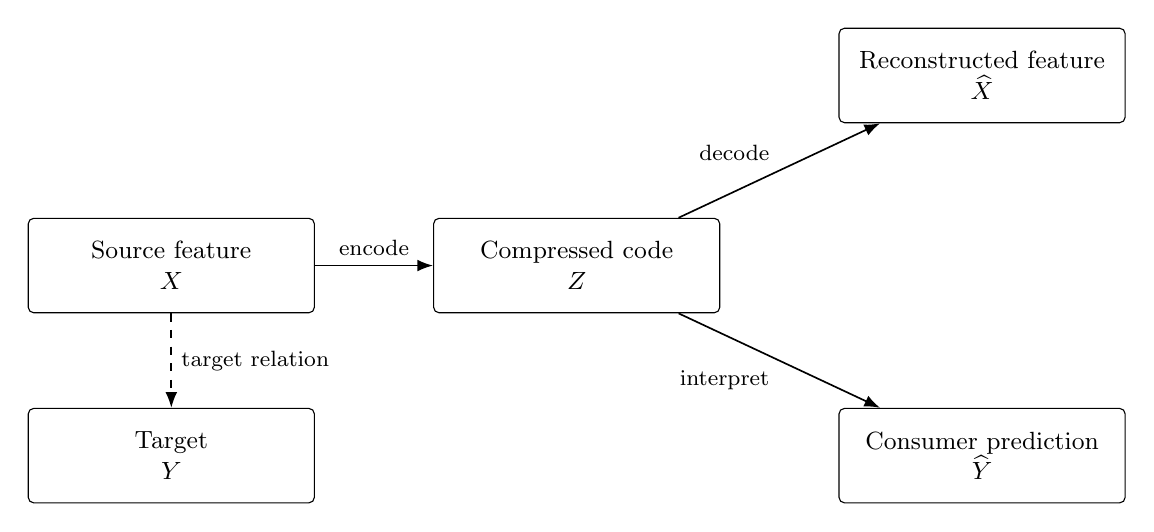
\begin{tikzpicture}[
    node distance=12mm and 15mm,
    box/.style={draw, rounded corners=2pt, align=center, text width=34mm, minimum height=12mm, font=\small},
    arr/.style={-{Latex[length=2mm]}, semithick},
    lab/.style={font=\footnotesize, align=center}
]
\node[box] (source) {Source feature\\$X$};
\node[box, right=of source] (code) {Compressed code\\$Z$};
\node[box, above right=of code] (reconstruction) {Reconstructed feature\\$\widehat X$};
\node[box, below right=of code] (answer) {Consumer prediction\\$\widehat Y$};
\node[box, below=of source] (target) {Target\\$Y$};
\draw[arr] (source) -- node[above, lab] {encode} (code);
\draw[arr] (code) -- node[above left, lab] {decode} (reconstruction);
\draw[arr] (code) -- node[below left, lab] {interpret} (answer);
\draw[arr, dashed] (source) -- node[right, lab] {target relation} (target);
\end{tikzpicture}
\caption{Two uses of a compressed representation. Reconstruction assesses the recovery of source features, and downstream evaluation assesses the consumer's predictions. The dashed edge shows the target relation assumed by the information bottleneck, under which $Y$ depends on $Z$ only through $X$. Their performance rankings need not agree. The diagram expresses the distinction used in the argument and does not reproduce a particular model architecture.}
\label{fig:representation-routes}
\end{figure}

\section{Correction That Fits the Learner}

The second paper concerns the interface through which information reaches a learner. Li and colleagues build a unified discrete diffusion model for visual understanding and generation and transfer capabilities into it from teachers of a different kind, an autoregressive vision-language model for understanding and a continuous flow model for image editing \cite{li2026}. The model generates blocks of tokens in parallel and refines them over steps, whereas an autoregressive teacher predicts one token from its left context. This difference is the whole difficulty.

The paper's illustration is simple. Suppose the student's answer is ``Jason visited San Francisco'', and consider the partially completed state in which the first word of the city is masked and ``Francisco'' is already visible. An autoregressive teacher conditioned on the first words may assign high confidence to ``New''. That is a reasonable preference in the teacher's setting and a poor target in the student's, since it pushes the student toward ``New Francisco''. The earlier method for distilling an autoregressive model into a diffusion one copies the teacher's scores directly to the student's diffusion predictions \cite{su2026}. Applied between a larger, stronger teacher and a student that already has its own distribution, the authors find that this directly damages the student. On MathVista the base student scores 71.5 and the directly distilled student 47.7. The damage is not confined to one benchmark: in the paper's reasoning table, all seven benchmarks fall from the base row to the naive on-policy distillation row, for instance Geometry3k from 54.4 to 23.0 and MathVision from 35.8 to 17.9.

The remedy is an intermediary. Block size one reduces the model to an autoregressive model, so the same student can be used in two modes. Its autoregressive mode is trained on its own rollouts against the teacher, and its diffusion mode is then trained to agree with its own autoregressive predictions on randomly masked versions of those rollouts. Writing $p_s^{\mathrm{AR}}$ and $p_s^{\mathrm{Diff}}$ for the student's two views and $p_t^{\mathrm{AR}}$ for the teacher,
\begin{equation}
\mathcal{L}_{\mathrm{und}}
= D_{\mathrm{KL}}\!\bigl(p_s^{\mathrm{AR}} \,\|\, p_t^{\mathrm{AR}}\bigr)
+ D_{\mathrm{KL}}\!\bigl(\operatorname{sg}[p_s^{\mathrm{AR}}] \,\|\, p_s^{\mathrm{Diff}}\bigr),
\end{equation}
with the second term evaluated only at masked positions and the stop-gradient written $\operatorname{sg}$. The student's own distribution is the bridge between a teacher that speaks left to right and a student that must also speak into gaps. With this method MathVista rises to 77.0, and the ablations clarify why. Using the consistency term alone collapses to an accuracy of 24.1, since two views of one model supervising each other have nothing external to anchor them. Rollouts drawn from the student's diffusion mode fail where rollouts from its autoregressive mode succeed, because the autoregressive scores are then conditioned on contexts the student itself produced. A small nonzero sampling temperature improves the diffusion view, at 74.8 for a temperature of 0.4 against 73.9 for greedy rollouts, while greedy rollouts give the best autoregressive score. Perhaps most pointed for the present argument, an alternative and stronger teacher, Kimi K-2.6, scores 88.9 on MathVista against 82.7 for the Nemotron teacher, yet distillation from it yields 71.6 against 78.1. The authors attribute this to the larger gap between teacher and student, including a different tokenizer and a different format for reasoning traces, in experiments they describe as early and not directly comparable to the others.

The image editing branch applies a related principle to a continuous teacher, for which distribution matching is unavailable, so the divergence terms and stop-gradient of the language branch have no direct analogue here. The student produces an edited image, which is re-encoded into the teacher's latent space, partially noised with strength $r$, and denoised by the teacher over several steps. The refined image becomes a training target. The authors are explicit that this is supervised learning on teacher-refined targets and not on-policy distillation in the strict sense, although the target is derived from the student's own output. On ImgEdit the base student scores 3.81, training on independently generated teacher images gives 3.90, and training on teacher-refined student outputs gives 4.17. The noise strength matters in an instructive way: $r = 0.9$ is best, and $r = 1.0$, where the starting point carries no trace of the student's attempt, falls to 3.90, the same score as the independent-generation baseline. The authors also observe that refinement can beat the teacher's own generation, because constraining the teacher to the neighbourhood of the student's attempt limits its tendency to over-edit.

Two further features of the paper bear on the economics. The model uses an elastic mixture-of-transformers design in which a task loads only the parameters it needs, so that understanding runs on an 8B branch and generation on 12B, with the full 16B reserved for interleaved tasks. Decoding speed trades against accuracy through a confidence threshold: roughly 553 tokens per second at 75.0 on MathVista against 203 tokens per second at 76.1 for autoregressive decoding (both reported per accelerator on H100 hardware in the paper's speed table, an exchange of about 2.7 times the throughput for 1.1 points), and about 998 tokens per second at 73.4 under a looser threshold. The cost of obtaining the capability is of another order. Training used 64 H100 accelerators over 26 days, about 40{,}000 accelerator-hours, of which the distillation stage took five days, and the language distillation still requires teacher and student to share a vocabulary. The model and code are released, so a downstream user consumes the result and does not reproduce it.

The broader architectural lesson is a hypothesis to be tested, and not a conclusion the paper reaches. Correction may be more effective when it addresses the learner's particular attempt and is translated into the learner's own predictive context. The paper supports this as an engineering mechanism for these tasks. It does not show that the pattern transfers to programming or to document research, and the authors name tokenizer matching as an open limitation.

\section{Experience Cards, Adapters, and the Cost of Using What Was Learned}\label{sec:hamo}

A third line of evidence concerns what happens after an agent has solved a problem once. The harness--model collaboration study of Bi and co-authors \cite{bi2026} addresses long-horizon agents that repeatedly meet related multi-step tasks, and it separates the retention of experience from the competence to use it. Each successful expert trajectory is distilled by a language model into an experience card consisting of the task description, the initial observable conditions, and a strategy-level outline of the solution. The cards accumulate in a persistent external memory, so that a newly acquired strategy is available at the next task without any change to the model. A single low-rank adapter on a frozen backbone is then trained, across successive stages, to act under the guidance of a retrieved card, using the same arrangement of request, initial observation, and injected experience at training time and at inference time. The authors' reason for the second component is that retrieval supplies guidance without supplying the ability to apply it: the model must still identify which objects in the present environment correspond to those in the card, decide whether the advice applies, and translate it into actions. Their case study illustrates the point. When a card advises rechecking requirements against the present task, the adapted agent notices that a candidate product's title does not establish the requested flavour, attempts to select the option, and verifies the price against the stated budget before purchasing, whereas the unadapted base model buys the mismatched product immediately. The authors themselves note that the case does not isolate which component produced the improvement.

The reported results support the combination within the environments studied. On ScienceWorld with an 8B backbone, the score rises from 38.13 after the first stage to 60.49 after the fourth, with a four-stage average of 52.22 against 38.34 for the harness alone, and the 14B backbone behaves similarly, with an average of 53.09. In the cross-domain stream from ScienceWorld through ALFWorld to WebShop, the final scores on the three domains are 52.43, 66.79, and 59.64, and two trajectory-training baselines fall on the earlier domains well below the unadapted backbone while improving on the last, so that adaptation to the latest domain does not by itself ensure retention of the earlier ones. A parameter-only baseline obtains a higher ALFWorld score (69.34 against 66.79) but its ScienceWorld score falls from 53.98 after the first stage to 24.57 after later training, whereas the combined system finishes at 52.43. The retention benefit therefore comes with a tradeoff on acquisition for one domain, and the paper's own limitations section states that forgetting is mitigated and not eliminated. The comparison is also confounded in the way that matters for an economic reading. The parameter-only baseline omits both the external memory and the replay of earlier trajectories, which the combined system retains, and replay alone can reduce forgetting, so the experiment supports the package and does not apportion credit among memory, replay, anchor selection, and experience conditioning. The authors list controlled ablations of these components among their future work.

For a resource-constrained research programme the more instructive element is the selection mechanism. Training on every stored trajectory would make the cost of parameter updates grow with the archive, and many trajectories express the same strategy. The method therefore embeds the cards, retrieves for each card its three nearest neighbours within the candidate collection excluding itself, and inverts that relation: the set $R_j$ of cards whose neighbourhoods contain card $j$ measures how many other situations the strategy of card $j$ could serve. A card is not selected for its retrieval count alone, because two heavily retrieved cards may serve nearly the same queries. Selection is instead greedy on marginal coverage, taking at each step the card whose retrieved set adds the most queries not already covered by the selection, until the marginal coverage reaches zero, and the number of cards actually used for training is set at the knee of the resulting coverage curve. Every card remains available for retrieval, and the optional release of memory entries after training is disabled in all reported experiments. The point for the present argument is that the training set is chosen by marginal coverage and not by taking the whole archive, so that training cost depends on the number of selected trajectories, their lengths, and the replay volume, and not directly on the number of stored cards. That number is itself determined by the archive, its neighbourhood structure, and the knee rule, and overlapping retrieval neighbourhoods are not equivalence classes, so coverage is a heuristic for avoiding redundancy and not a count of distinct situations.

Several properties of this procedure can be stated exactly, and SymPy is a convenient way to state and check them. The retrieval relation has a fixed total: with $M \ge 4$ cards and exactly three distinct neighbours per query, the hit counts satisfy $\sum_j n_{\mathrm{hits}}(j) = 3M$, so the mean count is three and a card is distinguished as broadly reusable only relative to that mean. The cost of a straightforward greedy implementation is also easily derived. If $M$ candidates are scanned at each of $N_s$ selection steps, and each step removes the chosen card from the pool, the number of marginal-coverage evaluations is
\begin{verbatim}
M, Ns, t = sp.symbols("M N_s t", integer=True, positive=True)
evaluations = sp.factor(sp.summation(M - t, (t, 0, Ns - 1)))
\end{verbatim}
which gives
\begin{equation}
\sum_{t=0}^{N_s - 1}(M - t) = \frac{N_s\,(2M - N_s + 1)}{2},
\end{equation}
so the exhaustive scan grows with the product of archive size and selection size, which is the reason the authors use lazy priority-queue updates that reuse stale marginal values as upper bounds. The expression also shows that when $N_s$ is a small fraction of $M$ the cost is close to $MN_s$ and the selection step is linear in the archive for a fixed training budget. These statements concern the counting model and not the paper's measured running time, which is not reported.

The adapter side of the cost can be treated in the same way. A rank-$r$ low-rank update to a weight matrix of shape $d_{\mathrm{in}} \times d_{\mathrm{out}}$ introduces $r(d_{\mathrm{in}} + d_{\mathrm{out}})$ trainable parameters against $d_{\mathrm{in}} d_{\mathrm{out}}$ for the full matrix:
\begin{verbatim}
d_in, d_out, rank, d, T = sp.symbols("d_in d_out r d T", positive=True)
fraction = sp.simplify(rank*(d_in + d_out)/(d_in*d_out))
square = fraction.subs({d_in: d, d_out: d})
illustration = square.subs({d: 4096, rank: 16})
\end{verbatim}
The fraction is $r/d_{\mathrm{in}} + r/d_{\mathrm{out}}$, which reduces to $2r/d$ for a single square matrix and equals $1/128$ for that individual weight matrix at the rank of 16 reported in the paper and the illustrative width of 4096. The fraction of the whole model depends on which matrices are targeted and on their dimensions. The paper's design also continues a single adapter from stage to stage instead of training one adapter per stage, so that the trainable budget stays constant, whereas a collection of $T$ retained adapters of equal size has $T$ times as many total adapter parameters, a ratio of exactly $T$ that compares storage and total parameters and not the number trained simultaneously. The adapter fraction is a statement about parameters and not about compute, since training still requires forward and backward passes through the frozen backbone on every selected trajectory, three epochs per stage at a learning rate of $2 \times 10^{-4}$, on NVIDIA A800 GPUs with 80 GB of memory. The paper reports no end-to-end measurements of the costs of card extraction, embedding, retrieval, replay, training, and inference, and it identifies such measurements as future work. It would therefore be a mistake to read the results as showing the system to be cheaper to operate, and the hardware shows that the work is not a demonstration of independence from accelerators.

\section{From Experience Cards to Checked Procedures}\label{sec:progression}

The collaboration study and the symbolic examples occupy different positions on a single scale of explicitness. An experience card is guidance in natural language that a model must interpret on every use. Its reuse cost includes the card's tokens in the prompt, the retrieval operation, and the model's inference over the card in the context of the present environment, and its reliability is the reliability of that interpretation. A symbolic expression that has been derived and checked is at the other end: once its assumptions are recorded and its transformation verified, it can become an ordinary function that requires no language-model interpretation, and the cost of each use is a small number of arithmetic operations. The collaboration study improves the model's ability to reuse a procedure that remains a procedure for the model to execute. Symbolic derivation can in some cases remove the model from the execution of that procedure altogether.

This suggests a progression for what a research system retains after a successful episode (Figure~\ref{fig:checked-reuse}), which is a proposal for design and is not a result of the paper. The first stage is a source-linked strategy description of the kind that the experience card already is, which is cheap to produce and has to be interpreted on each use. The second stage arises from repetition: when the same strategy is used on many tasks, its preconditions and operations can be inspected for stable structure, such as the fact that a purchase should follow a check of the stated constraints against the candidate's attributes. The third stage applies only where the stable operations admit formal expression. A constraint check can become a predicate over structured fields, a cost model a closed form, a transformation an identity verified by simplification, and an expected behaviour a test. The fourth stage is execution by conventional code, with the model retained for the cases the formalization does not reach, which are the ambiguous ones. A card that has passed through the first three stages is no longer an instruction to be interpreted. It has become a checked artefact whose cost of reuse is small relative to model inference, since execution no longer requires language-model interpretation, although a checked script can still be expensive if it searches or processes large inputs, and the verification effort is the overhead $s_j$ of the accounting section, repaid through a high reuse fraction $r_j$ on later tasks.

\begin{figure}[tbp]
\centering
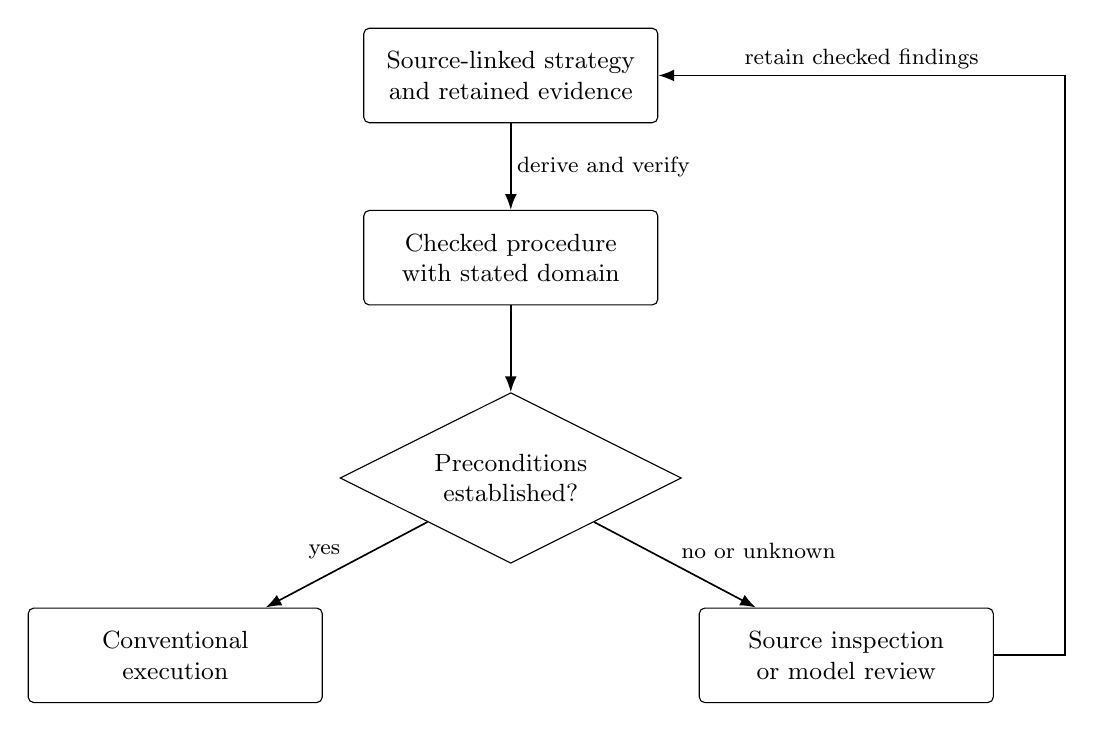
\begin{tikzpicture}[
    node distance=11mm and 13mm,
    box/.style={draw, rounded corners=2pt, align=center, text width=35mm, minimum height=12mm, font=\small},
    decision/.style={draw, diamond, aspect=2, align=center, inner sep=2pt, text width=27mm, font=\small},
    arr/.style={-{Latex[length=2mm]}, semithick},
    lab/.style={font=\footnotesize, fill=white, inner sep=2pt}
]
\node[box] (record) {Source-linked strategy\\and retained evidence};
\node[box, below=of record] (procedure) {Checked procedure\\with stated domain};
\node[decision, below=of procedure] (gate) {Preconditions\\established?};
\node[box, below left=of gate] (execute) {Conventional\\execution};
\node[box, below right=of gate] (review) {Source inspection\\or model review};
\draw[arr] (record) -- node[right, lab] {derive and verify} (procedure);
\draw[arr] (procedure) -- (gate);
\draw[arr] (gate) -- node[above left, lab] {yes} (execute);
\draw[arr] (gate) -- node[above right, lab] {no or unknown} (review);
\draw[arr] (review.east) -- ++(9mm,0) |- node[pos=0.75, above, lab] {retain checked findings} (record.east);
\end{tikzpicture}
\caption{Reuse through a checked procedure, with an explicit boundary for applicability. Unestablished preconditions lead to further inspection rather than unconditional execution. New findings return to the retained record and do not automatically modify the checked procedure.}
\label{fig:checked-reuse}
\end{figure}

The coverage idea transfers to this progression as a criterion for deciding where formalization effort should go. A strategy that is retrieved for many distinct situations is a better candidate for the expense of derivation and testing than one that covers only itself, and complementary coverage prevents the effort from being spent several times on strategies that differ only superficially. The same caution that the paper applies to its own proxy applies here. Retrieval coverage measured by embedding similarity is an estimate of usefulness and not usefulness itself, so a rare exception that is poorly represented by its neighbourhood can be important for correctness, and a procedure formalized from frequent cases can silently fail on exactly such an exception. Symbolic checking guards against errors of derivation within a stated model, and it does not guard against a model that omits the exceptional case. The disabled memory release in the experiments carries the corresponding warning about the end of the progression. The results do not show that learned competence can safely replace the external records from which it developed, and a system that discards a card after training an adapter, or discards a derivation after distilling it into a function, loses the ability to audit why the behaviour exists. Retaining the source-linked record beside the checked artefact is the conservative arrangement and is the one the experiments themselves adopt.

\section{Serving Efficiency and the Amount of Inference Required}\label{sec:serving}

Inference-serving frameworks introduce a further distinction into the resource argument. The SGLang repository \cite{sglang} describes an execution framework for language, vision-language, and diffusion models, optimized for agentic workloads, large-scale serving, and reinforcement-learning rollouts, with a surrounding ecosystem of deployment, routing, and orchestration integrations. Such infrastructure addresses how model computation is executed and shared across requests. A research harness addresses a related but different question, namely which requests should be made, with what context, and what should be retained afterwards. These responsibilities can overlap in an implementation, but their economic contributions should be measured separately. The assessment here rests on the repository's own description and not on any benchmark of the system, so it concerns the category of tool and not its measured performance. The system is named only as an example of that category and is neither evaluated nor endorsed.

A serving improvement can lower the execution cost of a prescribed workload without changing the number of questions that workload asks. A symbolic derivation can instead change the workload itself, replacing repeated model-mediated reasoning with an ordinary calculation. Retained evidence can eliminate another request, and a sufficiently informative representation can reduce the context that a remaining request requires. These interventions operate at different places in the accounting and can reinforce one another. Let $Q$ denote the number of inference requests, let $\bar c$ be their average execution cost under a specified workload and deployment, and let $H$ include preparation, retrieval, verification, and infrastructure overhead. A simplified accounting is
\begin{equation}
C = C_{\mathrm{inf}} + H, \qquad C_{\mathrm{inf}} = Q\bar c .
\end{equation}
A serving improvement primarily targets $\bar c$, while changes to the research procedure can reduce $Q$ or alter the requests from which $\bar c$ is calculated. The separation is an approximation, because request lengths, concurrency, and reuse affect execution efficiency, so $\bar c$ is not an intrinsic constant of the model. Nevertheless, the expression prevents a throughput improvement from being mistaken for a reduction in the amount of reasoning the programme demands.

Suppose a deployment change reduces average execution cost by a factor $\gamma$, while the researcher expands the request count by a factor $\lambda$. Holding the request distribution fixed and setting aside changes in overhead, inference expenditure becomes
\begin{equation}
C_{\mathrm{inf}}' = \frac{\lambda}{\gamma}\,C_{\mathrm{inf}} .
\end{equation}
Expenditure falls when workload expansion remains below the efficiency gain, stays constant when the two factors match, and increases when the newly affordable workload expands faster. This is a conditional accounting statement and not a prediction of behaviour. It explains why a researcher who readily multiplies worthwhile experiments can benefit from faster serving while continuing to encounter the same budget constraint. The same algebra gives the scale at which adopting a serving layer pays. If adopting it carries a one-time overhead $s_d$ for installation, configuration, and maintenance, and reduces execution cost by the factor $\gamma > 1$ at a fixed request count, the saving is $Q\bar c(1 - 1/\gamma)$ and the break-even request count is
\begin{equation}
Q^{*} = \frac{\gamma\, s_d}{\bar c\,(\gamma - 1)},
\end{equation}
which \verb|sp.solve| returns directly from the equality of overhead and saving. Below $Q^{*}$ the layer costs more than it saves, and the threshold rises with the overhead and falls with the per-request cost, so that a large serving framework is justified by a large and sustained request volume and is not justified merely by its capability.

The hardware question is similarly specific. The repository lists execution paths spanning accelerators, CPUs, and Apple Silicon, which shows that independence from a particular accelerator need not mean abandoning language models and can mean running a suitable model through another backend. Availability of a backend does not establish that a particular model will fit, that its required operations are supported, or that its latency will be useful. Independence from specialized accelerators should therefore be evaluated as a property of a complete workload: the model, its representation, the execution backend, and the frequency with which inference remains necessary. The relevant research objective is to combine efficient execution with durable reductions in repeated work. Serving infrastructure makes the remaining calls more economical, whereas symbolic derivation, checked procedures, and retained evidence determine how many calls remain, and their combined evaluation should report useful verified results per unit of total expenditure, including the overhead required to obtain those results.

\section{Defaults, Dependencies, and the Order of Reliance}\label{sec:defaults}

The break-even calculation for a serving layer is an instance of a general question about how much machinery a research system should depend on, and the symbolic and numerical examples above suggest an order of reliance. The first tier consists of the facilities of the language itself, such as arithmetic, comparison, iteration, and the standard library, whose behaviour is documented and stable, and which are exercised by a very large number of programs, although not necessarily by every program. The second tier consists of widely used and heavily tested packages that supply a bounded capability, of which SymPy, pandas, and SQLite are examples used here. The third tier consists of frameworks, which differ from libraries in the direction of control: a library is called by the programme, whereas a framework calls the programme's code through its own conventions, lifecycle, and configuration, and the programme must therefore be arranged to fit it. Web application frameworks of the Django type and serving frameworks of the kind discussed above belong to this tier, and so do agent harnesses. Each tier adds capability and adds overhead of the kind that the accounting section denotes $s_j$, namely the effort to learn the conventions, to configure the system, to follow its changes, and to diagnose the interactions among its parts, and the justification for a higher tier is the standard one, that the overhead is smaller than the work it spares. The order of reliance recommended by this reading is to establish a solution with the lower tiers first and to adopt a higher tier when a measurement shows that the lower tiers cannot meet the requirement at acceptable cost.

A related practice is to use the default configuration of a tool wherever possible, as with an editor used without plugins or a shell used without customization, so that the working environment is the same as the one obtained on a fresh machine. Three reasons suggest that a restrained configuration policy is worth investigating. The default configuration is plausibly the one exercised by the largest number of users, although that is not invariably so, and to that extent its failures are more likely to have been found and documented. A system with fewer configured elements has fewer interactions among them, and the number of potential pairwise interactions among $n$ elements grows quadratically, as $n(n-1)/2$, in the manner of the comparison counts in the cost examples above, which is an analogy and not an identity, since two configured tools interacting is not the same as two items being compared. An environment that departs from the defaults only where a documented need exists can be reproduced from a short specification, which lowers the cost of moving work to another machine and of returning to it after a long interval. The practice is a form of the essay's own principle, since a default is a retained artefact whose verification has been paid for by others and whose reuse fraction is high.

The reasons are plausible and are not established here, and the practice has costs that the same accounting makes visible. Functionality that a higher tier already provides must be rebuilt or forgone, a lower-tier solution may be slower or more error-prone than a mature package for the same capability, and a convention that is widely used can still be wrong for a particular task. The absence section illustrates both sides. The missing-value conventions of each tool are defaults, they differ from one tool to the next, and every layer added between a datum and its use is another place at which the convention can change without notice, so that a minimal chain of tools keeps the number of such transitions small. At the same time the conventions are not interchangeable, and a default that suits one stage can silently alter the meaning of another. The effect of a minimal-dependency discipline on reliability is therefore a measurable hypothesis. Candidate measurements are the time to reproduce a working environment on a fresh machine, the number of configuration items that depart from defaults and the fraction of observed failures traceable to them, and the effort per dependency in updates and diagnosis compared with the work that dependency spares. None of these has been measured for the systems discussed in this essay.

\section{Where Expensive Inference Belongs}

Taken together, these considerations make the central design problem one of allocation: deciding where expensive inference contributes information that cheaper procedures cannot reliably supply. Repeated parsing, exact comparison, indexing, and established checks often admit conventional implementations that run on ordinary processors. Ambiguous interpretation and unresolved conceptual relationships may require a language model. The boundary should remain empirical, because a cheap procedure that silently destroys relevant distinctions imposes costs downstream that the cheap stage never reports. The Proposition and the representation evidence both say this: a lossy stage is safe only relative to the questions that follow it.

The correction evidence adds a second consideration: indiscriminate escalation can itself be a failure, as the teacher-choice ablation illustrates, although that is a single instance and not a general result. Sending more tasks to a stronger model raises expenditure without guaranteeing that the surrounding system can assimilate what comes back. A correction is useful when it becomes something the system can apply, verify, or retain. In a document pipeline, the analogue of teacher refinement would be for a strong model to inspect a cheap procedure's draft extraction and edit it within a constrained neighbourhood of that draft, and not to regenerate the extraction from scratch, since a result anchored to the draft is both cheaper to check and more likely to be absorbed by the stage that produced it. The analogue of the noise-strength finding is that an edit with no trace of the draft is simply an independent generation with a refinement label. The analogue of the confidence threshold is the point at which the cheap stage hands an item upward. These analogies are proposals for testing and carry no evidential weight of their own.

A harness becomes valuable when it manages this allocation well, and its evaluation should reflect that. The relevant quantities include how much context it avoids resending, how effectively it retrieves prior results, how clearly it identifies unresolved questions, and how often a model-generated procedure becomes independently checkable. Orchestration overhead can be justified by reduced repetition or improved reliability, but the benefits have to be weighed against the whole workload, in the manner of the accounting above.

The archive itself should accumulate more than generated prose. It can retain source-linked claims, explicit assumptions, definitions, failed conjectures, verified transformations, and executable checks. These artefacts let later work begin from established results, and they make uncertainty visible, so that an unsupported inference does not become an apparently settled premise merely through repetition. In terms of the cost model, they are what raises the reuse fractions $r_j$, and the verification and linking that produce them are the overhead $s_j$. The overhead is acceptable only if the checks are cheaper than the work they allow later investigations to skip.

\section{A Programme of Measurement}\label{sec:measure}

Because the argument is conditional on empirical quantities, it suggests a short list of measurements that could be taken on a real archive, described here in prose so that each can be run independently.

The first is cost per retained verified claim, meaning the tokens spent, including orchestration, divided by the number of claims that end the process linked to a source, checked, and reusable. This replaces cost per task, which rewards a harness for producing many unverified outputs. The second is the realized reuse fraction $r_j$ across successive investigations, defined through the fraction of baseline cost avoided and not through the fraction of questions answered from stored artefacts, since answering nine inexpensive questions from memory while recomputing one expensive result yields high apparent reuse and little saving. The estimate therefore requires matched task costs or a specified counterfactual baseline, and the costs of retrieval, of checking applicability, and of invalidating stale artefacts have to be included on the side of the overhead $s_j$. A programme in which $r_j$ stays near zero is not accumulating structure however much it produces.

The third is a purpose-indexed measure of distinction loss. For each compressed record form, a set of probes is written from the original sources, covering questions that depend on qualifications, theorem conditions, and provenance, and the rate at which the compressed form fails them is compared with the failure rate of the full source. This is the archival counterpart of the divergence between reconstruction error and understanding, and it prevents a similarity score to the original from standing in for fitness for use. Representations made at several levels of resolution, from a coarse summary down to the source passage, could each be assigned the probe sets they are meant to serve, and the descent from one level to the next could be triggered by failure of a probe. The coarse-to-fine corruption schedule in the diffusion paper, in which tokens pass through intermediate states of increasing information before being fixed, is a loose precedent for treating commitment as graded and not binary, though nothing in the paper concerns archives.

The fourth is the correction-fit comparison. For a fixed set of items, a cheap procedure's drafts are corrected by a stronger model in two ways, constrained editing of the draft and independent regeneration, and the two are compared on downstream accuracy, on the size of the edits, and on the tokens spent. The noise-strength results suggest that the first should dominate when the draft is mostly right and that the two should converge as the draft worsens. The fifth is an escalation curve. The confidence threshold at which the cheap stage defers is varied, and accuracy is plotted against the tokens spent in the strong stage. The speed and accuracy table of the diffusion paper has this shape, and the same shape here would identify the operating point at which further escalation stops paying.

A sixth measurement concerns the progression of Section~\ref{sec:progression}. For each retained strategy, the tokens and latency of a use are recorded at each stage of explicitness, from a card interpreted by a model, through a checked formula or script, to conventional execution, together with the agreement rate between the stages on a fixed set of tasks and the verification cost that produced the later stages. A strategy is worth promoting when its agreement is high, its exceptions are enumerated, and the saved cost per use multiplied by the expected number of uses exceeds the verification cost, which is the break-even condition derived symbolically in the section on symbolic computation. The coverage count of the harness--model study provides a candidate way of ranking strategies for promotion, and the measurement would show whether that proxy tracks realized reuse.

A seventh measurement concerns absence, in the sense developed in Section~\ref{sec:absence}. Probes are drawn from the sources so that a known fraction of the questions have no attested answer, of several kinds, namely unattested, inapplicable, and premise-false cases. A contradicted proposition is treated separately, since it may have an attested negative answer and then calls for that answer and not for abstention. Each stage of a pipeline is then scored on the rate at which it returns an explicit absence of the matching kind and not a value, and on the rate at which a filled answer can be distinguished from a determined one by its recorded provenance. The measurement would show whether the analogy between missing-value conventions and model completion describes behaviour or only resembles it.

\section{What the Evidence Does Not Show}

Several limits should be stated plainly. Two of the papers concern visual understanding and generation, and the third concerns interactive agent benchmarks. None addresses text archives, programming, or mathematical research, and the extension of their lessons to those settings is a hypothesis. The semantic fidelity paper measures fidelity through benchmark averages, which sample particular demands and can hide differing failures, and its central comparisons come without uncertainty estimates. Its title asks about lossless representation, but the experiments establish a narrower result, that a discrete interface can match a continuous one on the average of a chosen benchmark suite at a large bit budget. The distillation paper credits much of its broad understanding improvement to additional training data and states that its text-to-image generation was not distilled because the base model already exceeded the candidate teachers. Its image-editing method is not on-policy in the strict sense, and it requires matched vocabularies for language distillation. Its speed gain is real and comes at a measured loss of accuracy. The harness--model study concerns text-based agent benchmarks, reports no end-to-end cost measurements, uses A800 accelerators, disables the release of memory entries in every experiment, and compares its full system with a parameter-only baseline that lacks both memory and replay, so it supports the combination as a package without apportioning credit among its components or showing that the combination is cheaper to operate. The progression from experience cards to checked procedures proposed in Section~\ref{sec:progression} is a design suggestion that no experiment in that paper tests. The discussion of serving frameworks in Section~\ref{sec:serving} rests on a repository description and no benchmark, and the argument for minimal dependencies in Section~\ref{sec:defaults} is a hypothesis with no measurement behind it. The comparison of missing-value conventions in Section~\ref{sec:absence} rests on behaviour exercised in the Python, pandas, SQLite, SymPy, R, and Julia implementations, and its extension to model completion is an analogy that none of the three papers measures.

Independence from specialized accelerators is the most speculative element of the motivating aim. The capabilities discussed here were produced with training budgets far beyond a single machine, and a local operator would consume released weights. What remains within reach is reducing the number and size of the calls made against such models, and shifting routine work to conventional procedures wherever a measurement shows that doing so loses nothing the downstream questions need. Whether that is possible for a given task is a measurement, not a premise.

\section{Computation That Leaves Structure Behind}

Research-scale capability remains expensive if every new question requires the whole process to begin again. A more sustainable programme turns computation into durable structure. Formal writing contributes by establishing, before any run, which questions the available representations can answer at all, which iterations collapse to closed forms, which searches can be pruned, and which implementations cannot meet their stated aims. Representation research contributes the reminder that preservation is relative to a consumer, so that archives should be compressed for stated purposes and checked against probes derived from those purposes. Distillation research contributes the observation that a stronger source of correction can damage a learner when its output is imposed in the wrong form, and can help when it is mediated by the learner's own predictions. Work on harness--model collaboration contributes the distinction between storing a procedure and being able to apply it, and the progression from interpreted cards to checked formulas, scripts, and tests carries that distinction to the point at which repeated reasoning is replaced by ordinary computation. Each expensive intervention should, where possible, leave behind something that reduces the cost or increases the reliability of the next investigation, and the measurements of the previous sections are a way of checking whether it did. The organizing principle of the essay is the inequality of the accounting section, under which retention pays when the total overhead of verifying and linking artefacts is smaller than the total work that later investigations are spared, and every section above is an account of how one side of that inequality might be raised or the other lowered.

\appendix

\section{Error Bound for Tight-Frame Synthesis}

Let $A \in \mathbb{R}^{Ld \times D}$ satisfy $A^{\top}A = \rho I_D$ with $\rho = Ld/D$, let $u = Az$ be the stacked projected views of a feature $z$, and let $q = u + e$ be the stacked quantized views, with $e$ the stacked quantization error. The synthesized feature is $\hat z = \rho^{-1}A^{\top}q$. Since $\rho^{-1}A^{\top}u = \rho^{-1}A^{\top}Az = z$, we have $\hat z - z = \rho^{-1}A^{\top}e$. Because $A$ has full column rank, $\rho^{-1}A^{\top}$ is a left inverse of $A$, and the $D$ singular values of $A$ all equal $\sqrt{\rho}$, so that the left inverse $\rho^{-1}A^{\top}$ has all singular values equal to $\rho^{-1/2}$. The quantized stack $q$ need not lie in the range of $A$, so the error is bounded through the operator norm and not by any orthogonality argument: $\lVert A^{\top}e\rVert_2^2 \le \rho\,\lVert e\rVert_2^2$, and therefore
\begin{equation}
\lVert \hat z - z\rVert_2^2 \;\le\; \frac{1}{\rho}\,\lVert e\rVert_2^2 .
\end{equation}
Analysis followed by synthesis recovers the original feature exactly before quantization, so all reconstruction error originates in replacing the projected views by their nearest codewords, which is the identity reported in the source paper \cite{zou2026}. The bound is a property of the geometry before and after quantization. It says nothing about which information the language model can extract from the indices, which is the separate question the representation section examines.

\begin{thebibliography}{99}
\sloppy

\bibitem{zou2026}
J.~Zou, X.~Li, Z.~Yue, X.~Huang, Y.~Luo, W.~Yan, H.~Li, W.~Liu, and X.~Wang.
Can Discrete Tokens Serve as Semantically Lossless Representations of Visual Signals?
\emph{arXiv preprint} arXiv:2610.37662, 2026.

\bibitem{li2026}
S.~Li, H.~Ye, G.~Heinrich, Y.~Fu, H.~Zhang, S.~Liu, A.~Grover, and P.~Molchanov.
Nemotron-Labs-Diffusion-Uni: Elastic Self-Refining Unified Diffusion LLM with Cross-Paradigm On-Policy Distillation.
\emph{arXiv preprint} arXiv:2610.36466, 2026.

\bibitem{bi2026}
Z.~Bi, Z.~Peng, Y.~Wang, X.~Chen, H.~Zhang, Y.~Zhang, Z.~Yang, Q.~Shen, and J.~Lou.
Harness--Model Collaboration for Long-Horizon Continual Learning.
\emph{arXiv preprint} arXiv:2610.34724, 2026.

\bibitem{meurer2017}
A.~Meurer, C.~P. Smith, M.~Paprocki, O.~\v{C}ert\'{i}k, S.~B. Kirpichev, M.~Rocklin, et~al.
SymPy: Symbolic Computing in Python.
\emph{PeerJ Computer Science}, 3:e103, 2017.

\bibitem{pandasna}
pandas Development Team.
Working with Missing Data.
User guide documentation, pandas 3.0, \texttt{pandas.pydata.org/docs/user\_guide/missing\_data.html}.

\bibitem{sqlitenulls}
SQLite Consortium.
NULL Handling in SQLite Versus Other Database Engines.
Documentation, \texttt{sqlite.org/nulls.html}.

\bibitem{numpyerrstate}
NumPy Developers.
Floating-Point Error Handling and \texttt{numpy.errstate}.
Reference documentation, NumPy 2.5, \texttt{numpy.org/doc/stable/reference/generated/numpy.errstate.html}.

\bibitem{juliamissing}
Julia Project.
Missing Values.
Julia manual, \texttt{docs.julialang.org/en/v1/manual/missing/}.

\bibitem{sglang}
SGLang Project Contributors.
SGLang: Fast Inference for LLMs and Multimodal Models.
Software repository and documentation, release v0.5.22, \texttt{github.com/sgl-project/sglang}.

\bibitem{futamura1999}
Y.~Futamura.
Partial Evaluation of Computation Process: An Approach to a Compiler-Compiler.
\emph{Higher-Order and Symbolic Computation}, 12(4):381--391, 1999.
Reprint of the 1971 paper. \url{https://doi.org/10.1023/A:1010095604496}.

\bibitem{tishby1999}
N.~Tishby, F.~C. Pereira, and W.~Bialek.
The Information Bottleneck Method.
In \emph{Proceedings of the 37th Annual Allerton Conference on Communication, Control, and Computing}, pages 368--377, 1999.
Preprint: \url{https://arxiv.org/abs/physics/0004057}.

\bibitem{elyaniv2010}
R.~El-Yaniv and Y.~Wiener.
On the Foundations of Noise-Free Selective Classification.
\emph{Journal of Machine Learning Research}, 11:1605--1641, 2010.

\bibitem{su2026}
X.~Su, J.~Helwig, S.~Parashar, A.~Chagi, L.~Jotsna, D.~Zhi, J.~Caverlee, D.~Kalathil, and S.~Ji.
Data-Efficient Autoregressive-to-Diffusion Language Models via On-Policy Distillation.
Preprint, 2026, as cited in the reference list of \cite{li2026}, which gives no identifier.

\end{thebibliography}

\end{document}

